\documentclass[basic,plain]{inVerba-notes}

\newcommand{\userName}{Cullyn Newman}
\newcommand{\class}{BI:\@ 337}
\newcommand{\theTitle}{Functions of Endoplasmic Reticulum}
\newcommand{\institution}{Portland State University}

\begin{document}

\chonk{Relevant Concepts} --- \textbf{Defects in the Permeability Barrier of Old NPCs}
\begin{itemize}
  \item Does the function of nuclear pore complexes become compromised in old cells?
    \begin{itemize}
      \item Findings in the paper thus far show that many nuclear pores do not get replaced in dividing cells, raising one of the central questions of this paper, i.e., the fate of the nuclear pores in postmitotic cells.
      \item Maintenance of the pores are important, as nuclear pore complexes help the nuclear membrane act as barriers, regulating the passage of molecules between the nucleus and cytoplasm thanks to its protein-lined channel. 
    \end{itemize}
  \item ``\dots a central role of the scaffold nucleoporins is to anchor other NPC components that are responsible for the maintenance of the nuclear permeability barrier\dots''
    \begin{itemize}
      \item This is what the authors decided to test, i.e., whether NPCs remain functional as cells age by inspecting membrane permeability, as intact should exclude molecules over a certain size.
    \end{itemize}
\end{itemize}

\medskip
\chonk{Techniques} --- \textbf{Fluorescent Dextrans and ``Leaky Nuclei''}
\begin{itemize}
  \item The authors used fluorescent dextrans with defined weights in order to inspect membrane permeability.
    \begin{itemize}
      \item Immunofluorescence is a technique for light microscopy that uses antibodies to target fluorescent dyes to chosen biomolecular targets, allowing for easy visualization.
      \item Fluorescent dextrans are hydrophilic polysaccharides that can have accurately defined weights, good water solubility, and low toxicity that have been labeled for viewing with immunofluorescence. These qualities of dextrans make them perfect for testing and visualizing permeability of nuclear membranes.
      \item The authors expanded on this with other techniques, such as WGA, in order to verify their findings, but I will just be illustrating how dextrans are used.
    \end{itemize}
  \item Shown in visualizations is how the authors exposed the membranes to dextrans that are both:
    \begin{itemize}
      \item[1.] slightly larger than max size of molecules excluded form intact nuclei (70 kDa vs.\ 60 kDa max limit).
      \item[2.] and dextrans much larger (500 kDa) to control for potential perturbation induced permeability that is outside the control of the nuclear pore complexes.
    \end{itemize}
  \item The results are hypothesized to demonstrate if older membranes become less selective, or ``leaky'', due to failure of maintenance as cells age if normally excluded size (70 kDa) is included.
\end{itemize}

\newpage 

\chonk{Illustration of Techniques} --- \textbf{Test of ``Leaky Nuclei''}
\bigskip

\begin{center}
  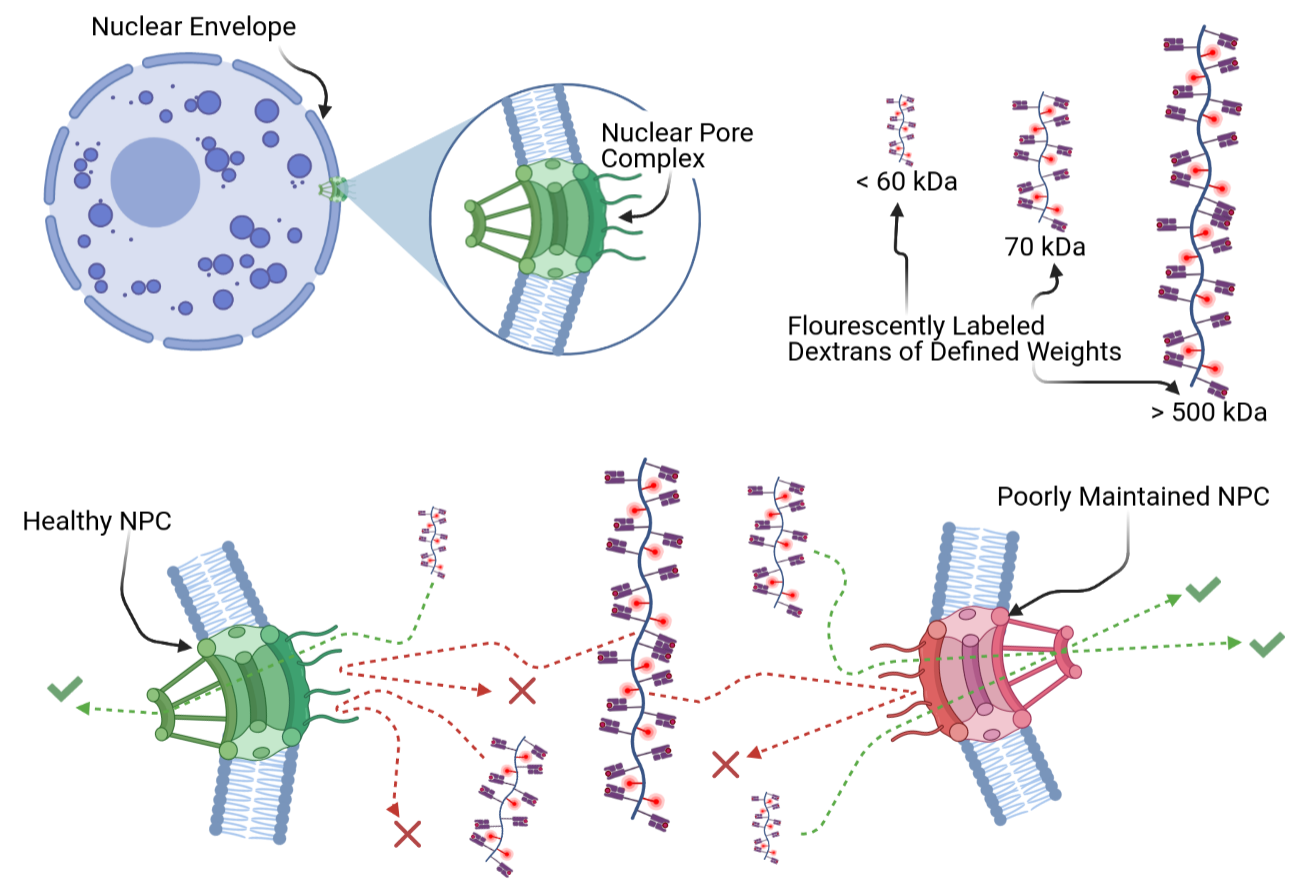
\includegraphics[width=\textwidth]{images/week-3-illustration.png}
\end{center}
\end{document}